\chapter{Track Finder Theory and Multivariate Classification} \label{chapter-theory}

The track finders are implemented in the Belle~II analysis software framework to which a short introduction is given here. More information can be found elsewhere~\cite{moll_basf2}. Afterwards, a more detailed description of the theory of track finding and common figures of merit for all track finders are explained and discussed. As some parts of the track finders rely on the usage of multivariate classification, the basic principle of boosted decision trees is described in the end of the chapter.

\section{The Belle~II Analysis Software Framework (basf2)}

For simulation, data acquisition, data processing and analysis of the Belle~II experiment basf2 is used. Although -- going by its name -- it seems to be built on top of the old software framework used for the Belle experiment, it is a complete rewrite of the software using modern programming principles in the programming languages C++~\cite{cpp} and Python~\cite{python}. Together with external libraries e.g.\ ROOT~\cite{root} or EvtGen~\cite{evtgen} this framework provides the basics for every software written for the experiment.

The software is divided into several packages -- each serving a distinct purpose or summarizing code for a single detector. Examples for packages are CDC, SVD or the tracking package which is described in more detail in chapters~\ref{chapter-workflow}.

Each use of basf2 -- e.g.\ simulation, reconstruction or analysis -- consists of processing one or more so called \emph{paths} filled with \emph{modules}. These modules perform a dedicated small task e.g.\ simulating the $\PUpsilonFourS$-decay (the \texttt{EvtGen} module), writing out data to a root file (the module \texttt{RootOutput}) or performing a track reconstruction (for example with the module \texttt{TrackFinderCDCAutomaton}). The presence, the order, and the parameters of the modules are determined in \emph{steering files} written with Python. The modules itself can be written in C++ or Python. 

In these steering files a path is created, filled with modules and passed to the framework which handles loading the corresponding C++ libraries and calling the modules for every event that should be processed. An example of a small steering file for track finding can be found in listing~\ref{lis-steering-file}. Due to this modular structure not only parallel processing but also debugging of intermediate steps can be performed easier.

Because many modules require the data produced by other modules as input, there is a need for intermodular communication. This communication is performed within the framework with the help of a data store. It is used in the framework to store e.g.\ the hit information produced by the particles in the simulation or the found tracks after the track finding modules. The modules have read and write access to every element in the data store -- accessors to receive from and put objects on the data store. Listing~\ref{lis-steering-file} shows an exemplary steering file. The visualization of the data flow between the modules created with this steering file can be found in figure~\ref{fig-viz-datastore}. The data store can be written to or read from disk using ROOTs own serialization mechanism together with data member dictionaries for the C++ classes created by the C++ interpreter of ROOT called CLING~\cite{cling}.

\begin{listing}
 \begin{lstlisting}[style=customP]
  # Import the needed basf2 package
  import basf2

  # Create a basf2 path
  path = basf2.create_path()

  # Add an input module to read from the file data.root
  path.add_module("RootInput", inputFileName="data.root")
  
  # Connect the gearbox, which is needed for loading the detector parameters
  path.add_module("Gearbox")

  # Add the Legendre track finder
  path.add_module("WireHitTopologyPreparer")
  path.add_module("CDCLegendreTracking", WriteGFTrackCands=False)
  # Add the stereo Legendre finder
  path.add_module("StereoHitFinderCDCLegendreHistogramming",
                  SkipHitsPreparation=True,
                  TracksStoreObjNameIsInput=True,
                  WriteGFTrackCands=True)
  
  # Save the data store to a root file
  path.add_module("RootOutput")

  # Process the path
  basf2.process(path)

 \end{lstlisting}
 \caption[Python steering file to create a typical basf2 path.]{Python steering file to create a typical basf2 path. After loading the needed Python libraries the path is created and filled with the modules. In the end, this path is processed and for each event the modules are executed in the given order and with their given parameters. For more information on the used modules see their documentation.}
 \label{lis-steering-file}
\end{listing}


\begin{figure}
 \centering
 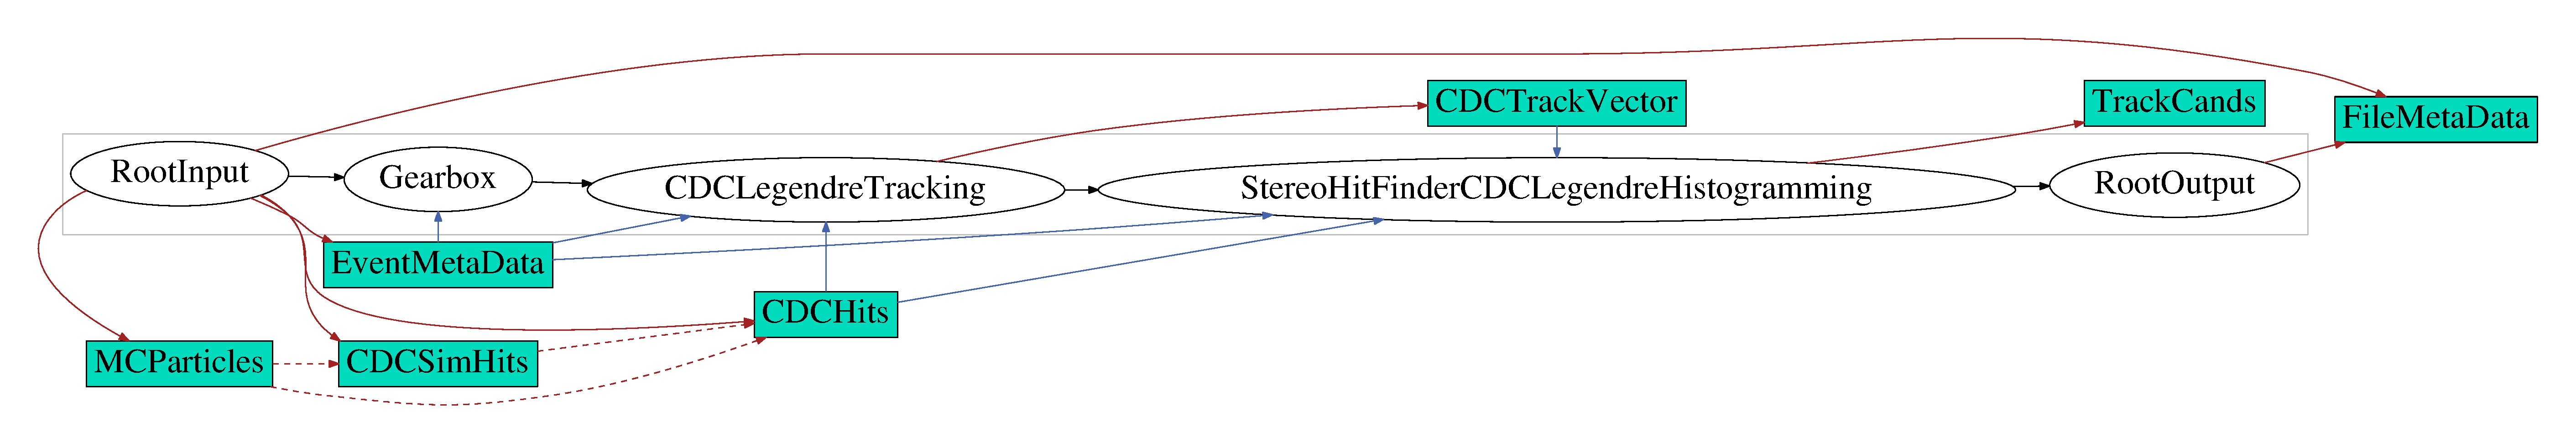
\includegraphics[width=\linewidth]{figures/theory/dataflow.pdf}
 \caption[Visualization of intermodular communication.]{Visualization of the intermodular communication while processing the path implemented with the steering file described in listing~\ref{lis-steering-file}. The green boxes are entries in the data store. The ellipses are the processed modules. The red and blue arrows depict input and output to the modules. The dashed lines relations between the entries on the data store.}
 \label{fig-viz-datastore}
\end{figure}


\section{Working Principle of the CDC Track Finder in basf2}

One part of this thesis was the improvement and further development of the track finder modules for the CDC tracking detector. Therefore, the working principles of the two track finders for this detector are described here briefly. For more information on the Legendre track finder see~\cite{kronenbitter}. More information on the automaton track finder can be found in~\cite{oliver}.

The general purpose of a track finding algorithm is to partition all measured wire hits into exclusive sets of hits that originate from the same charged particle passing through the detector. It does so by making several assumptions on the charged particles producing the wire hits, e.g.\ the helical form of their trajectory and therefore the possible patterns of the hits. By fitting a mathematical model of a trajectory to these hits one gains information on the momentum and position of this particle. This part is called track fitting and is described in section~\ref{section-fitting}. The sets of hits possibly belonging to a charged particle are called tracks in the following.

The reason to have two track finders for the CDC is their different ansatz. The Legendre track finder is a so called global track finder whereas the automaton track finder is a local one. A global algorithm uses the information of all wire hits simultaneously. The Legendre track finder does this by applying a mathematical transformation to the wire positions which should, in principle, project all hits belonging to the same track onto the same coordinates. It is insensitive to gaps in the hit pattern but rather sensitive to high energy loss of the particles and tracks with a large distance to the interaction point. A local algorithm however tries to use neighboring wire hits to construct clusters of hits. These clusters are then enlarged by using neighborhood relations again until a full track can be found. In opposite to a global track finding algorithm it can cope with energy loss, multiple scattering and displaced tracks more easily. In the following these two principles are described in more detail.


\subsection{The Legendre Track Finder}
The principle of using the Legendre transformation for tracking algorithms in high energy physics experiments was first described by Alexopoulos~\cite{legendre}. It uses an extended version of the Hough transformation introduced by Paul V.C. Hough in 1962~\cite{hough}. The algorithm uses the fact that each trajectory in the $r$--$\phi$-plane of the detector can be described by a circle -- assuming no energy loss -- because of the applied magnetic field in $z$ direction. In a first approximation one can also assume that each particle comes from the interaction point, which is valid for the bigger share of the decay products. Therefore the trajectory in the $r$--$\phi$ direction can be described by two parameters: the radius $R$ of the circle and the angle $\theta$ between an arbitrary, but fixed, axis and the tangent to the circle at the interaction point.\footnote{When dropping the last assumption (of tracks coming from the origin) one has to introduce another parameter -- often called $d_0$ -- which describes the minimal distance from the circle to the origin in the $r$-$\phi$ plane. It is easy to generalize the described algorithm to these three dimensions. At the moment, this third dimension is however not implemented in the tracking software as displaced tracks are found with the local track finder.}

Simplified, the idea is to calculate each trajectory that could have possibly created one of the axial hits and draw them all in a 2d histogram with the trajectory parameters $R$ (more precisely with $\rho = 1/R$) and $\theta$ as the coordinate axes. As there is only a small number of correct trajectories which are responsible for a great number of hits, there is a small parameter set which appears very often in the histogram. These parameters can then be identified and used to create tracks.

For applying this algorithm, the $x$ and $y$ coordinate pair of every axial wire hit together with the drift length $d$ is transformed by the functions
\begin{align} x' = \frac{2x}{x^2 + y^2 - d^2}\ , \qquad y' = \frac{2y}{x^2 + y^2 - d^2}\ ,  \qquad d' = \frac{2R}{x^2 + y^2 - d^2}\quad \text{and} \label{eq-inverse} \end{align}
\begin{align}\rho(\theta) = x' \cos(\theta) + y' \sin(\theta) \pm d' \label{eq-legendre}\end{align}
into the Legendre space as shown in figure~\ref{fig-legendre-explained}. In the first step of the transformation, the wire hits are transformed to the inversed plane. With the transformation in equation~\ref{eq-inverse} each circular trajectory through the interaction point is mapped onto a line. The two trajectory parameters $R = 1/\rho$ and $\theta$ are now functions of the slope and the axis intercep of this line. After that, each drift circle is transformed into a pair of sinusoidal functions -- also called sinograms. This function $\rho(\theta)$ in equation~\ref{eq-legendre} is constructed in a way to use the fact that each trajectory of a charged particle responsible for a wire hit must touch the drift circle tangentially. Each point on the constructed sinusoidal functions corresponds to one possible trajectory of a particle which could have created such a hit. There are two sinusoidal functions because the osculation point can be on the far or near side of the drift circle -- the trajectory circle can circumscribe the drift circle or not. This is also shown in figure~\ref{fig-sinusodial}.

\begin{figure}
 \centering
 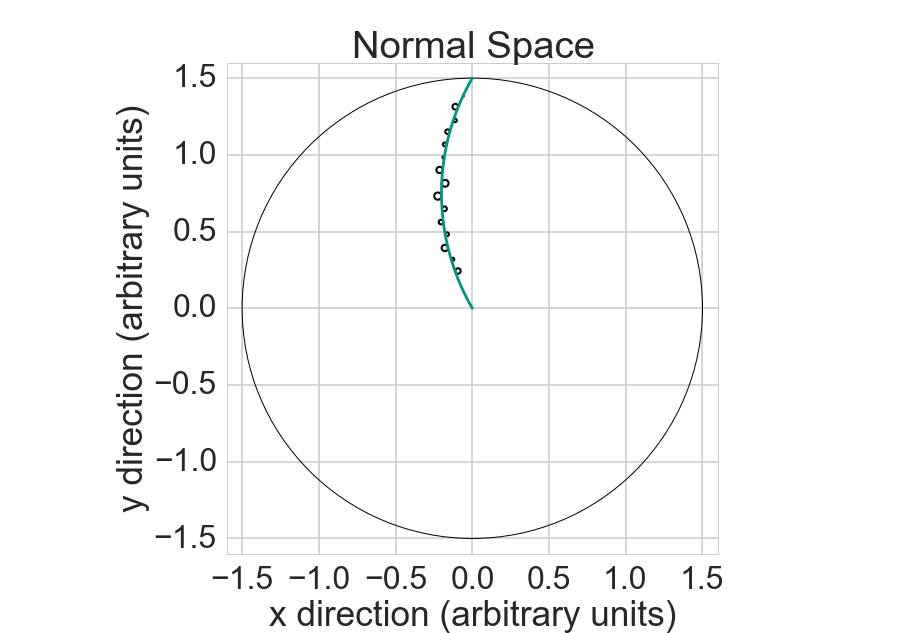
\includegraphics[scale=0.3]{figures/theory/legendre_1.png}
 \hspace*{1cm}
 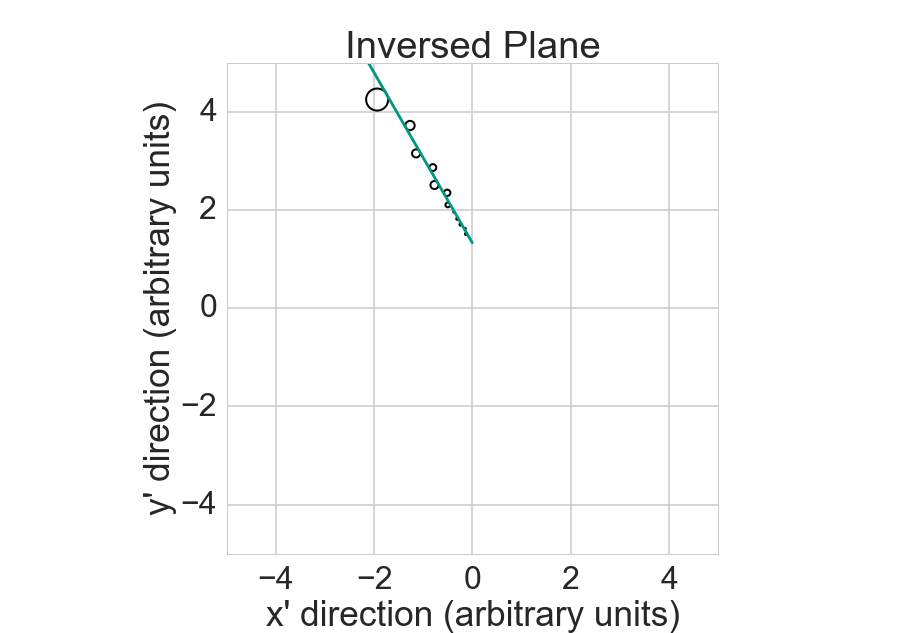
\includegraphics[scale=0.3]{figures/theory/legendre_2.png}
 
 \vspace*{1cm}
 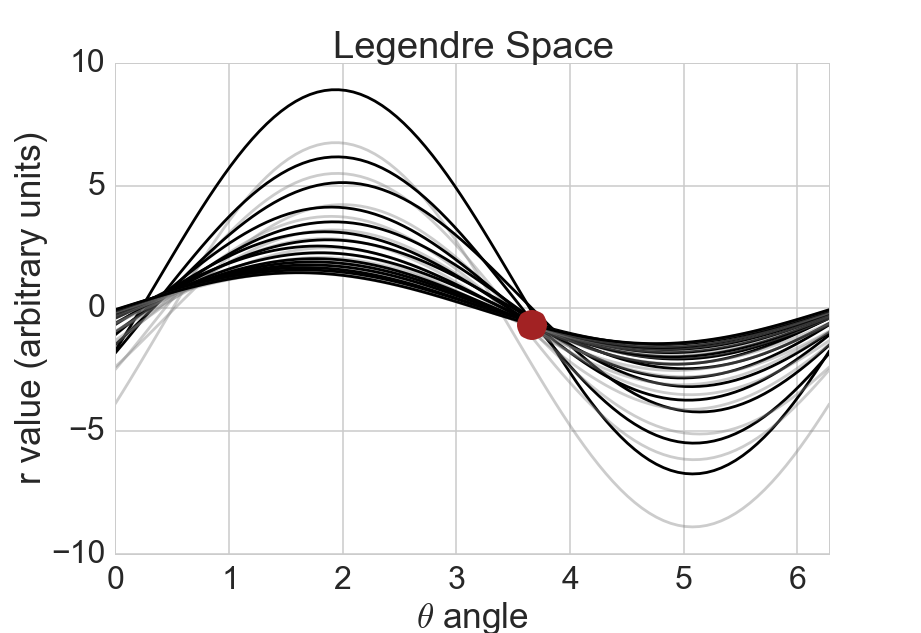
\includegraphics[scale=0.3]{figures/theory/legendre_3.png}
 \caption[Axial Legendre algorithm.]{Transformation of hits belonging to the same charged particle (upper left side) to the inversed plane (upper right side) and to the Legendre space with the characteristic sinusoidal functions (below). As described in the text, the circular trajectory is first transformed into lines and then into intersecting sinograms. Each sinogram includes all trajectory parameters possibly touching the hit from which the function was created. The intersection corresponds to the parameters of the trajectory and is marked with a red circle. For better visibility the wrong half of the sinograms is colored gray.}
 \label{fig-legendre-explained}
\end{figure}

\begin{figure}
  \centering
  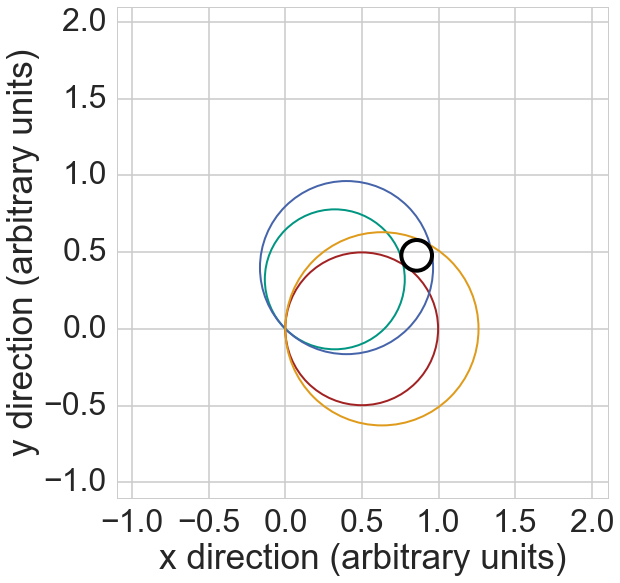
\includegraphics[scale=0.27]{figures/theory/sinosodial_1.png}
  \hspace*{1cm}
  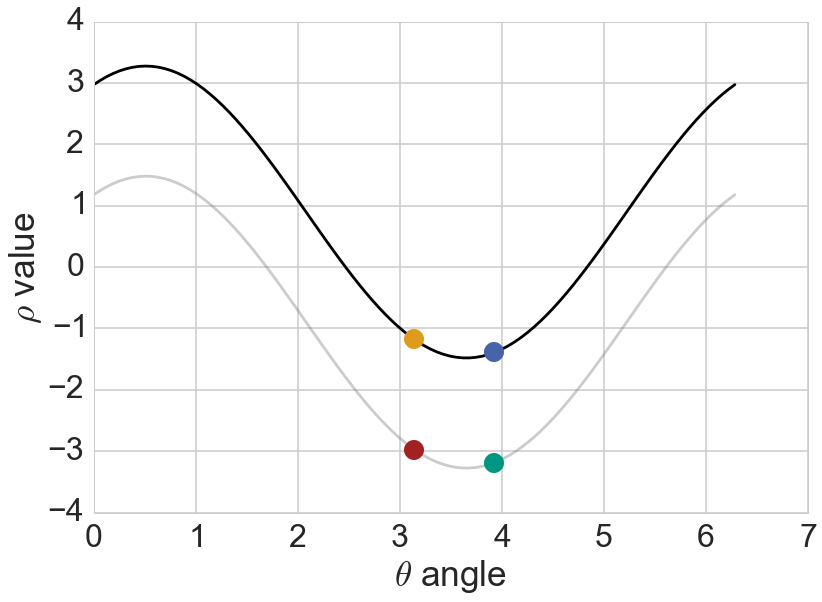
\includegraphics[scale=0.27]{figures/theory/sinosodial_2.png}
  \caption[Sinograms in the Legendre algorithm.]{The left picture shows one single oversized drift circle (black) and four trajectories (in color) that could have possibly created that hit as they touch the drift circle tangentially. The hit is transformed into two sinograms on the right picture. The drift circle lies on the outside of the green and red trajectories (gray sinogram = right side) and on the inside of the blue and yellow one (black sinogram = left side).}
  \label{fig-sinusodial}
\end{figure}


With using the information of a single hit one ends up with an infinite number of trajectory hypotheses. But as a charged particle passes many drift cells until it leaves the CDC detector -- in some cases up to 100 hits -- several wire hits are created with identical trajectory parameters. As these same parameters correspond to the same point in the Legendre space, the sinusoidal functions of the wire hits intersect in this point as can also be seen in figure~\ref{fig-legendre-explained}. The task of the Legendre algorithm now is to transform the hit coordinates and find those intersections.

Imperfections due to energy loss and material effects prevent the sinusoidal function from intersecting in one single point, but rather in a smeared area. To cope with this problem but still find intersections with a good performance a peak search in the binned Legendre space is applied. For each bin the number of sinusoidal functions passing this area is counted. The bin with the highest count is assumed to be the bin with the highest number of sinusoidal intersections. From the wire hits contributing to this bin a new track is created and the search is repeated with those hits deleted until a threshold in the bin entry is undercut. As the Legendre space is mostly empty, this procedure can be further improved in performance by refining the bin division from very coarse bin sizes to finer ones only for those bins which have a certain amount of sinusoidal functions in them. Because these bins are divided into 4 sub-bins with every refinement step the concept is called quad-tree search. The whole search is depicted in figure~\ref{fig-quad-tree-search}.

After finding possible hit subsets for the track candidates a post-processing procedure consisting of hit reassignment, hit deletion and track merging is applied to account for energy losses, trajectories not coming from the interaction point and finding inefficiencies.

\begin{figure}
  \centering
  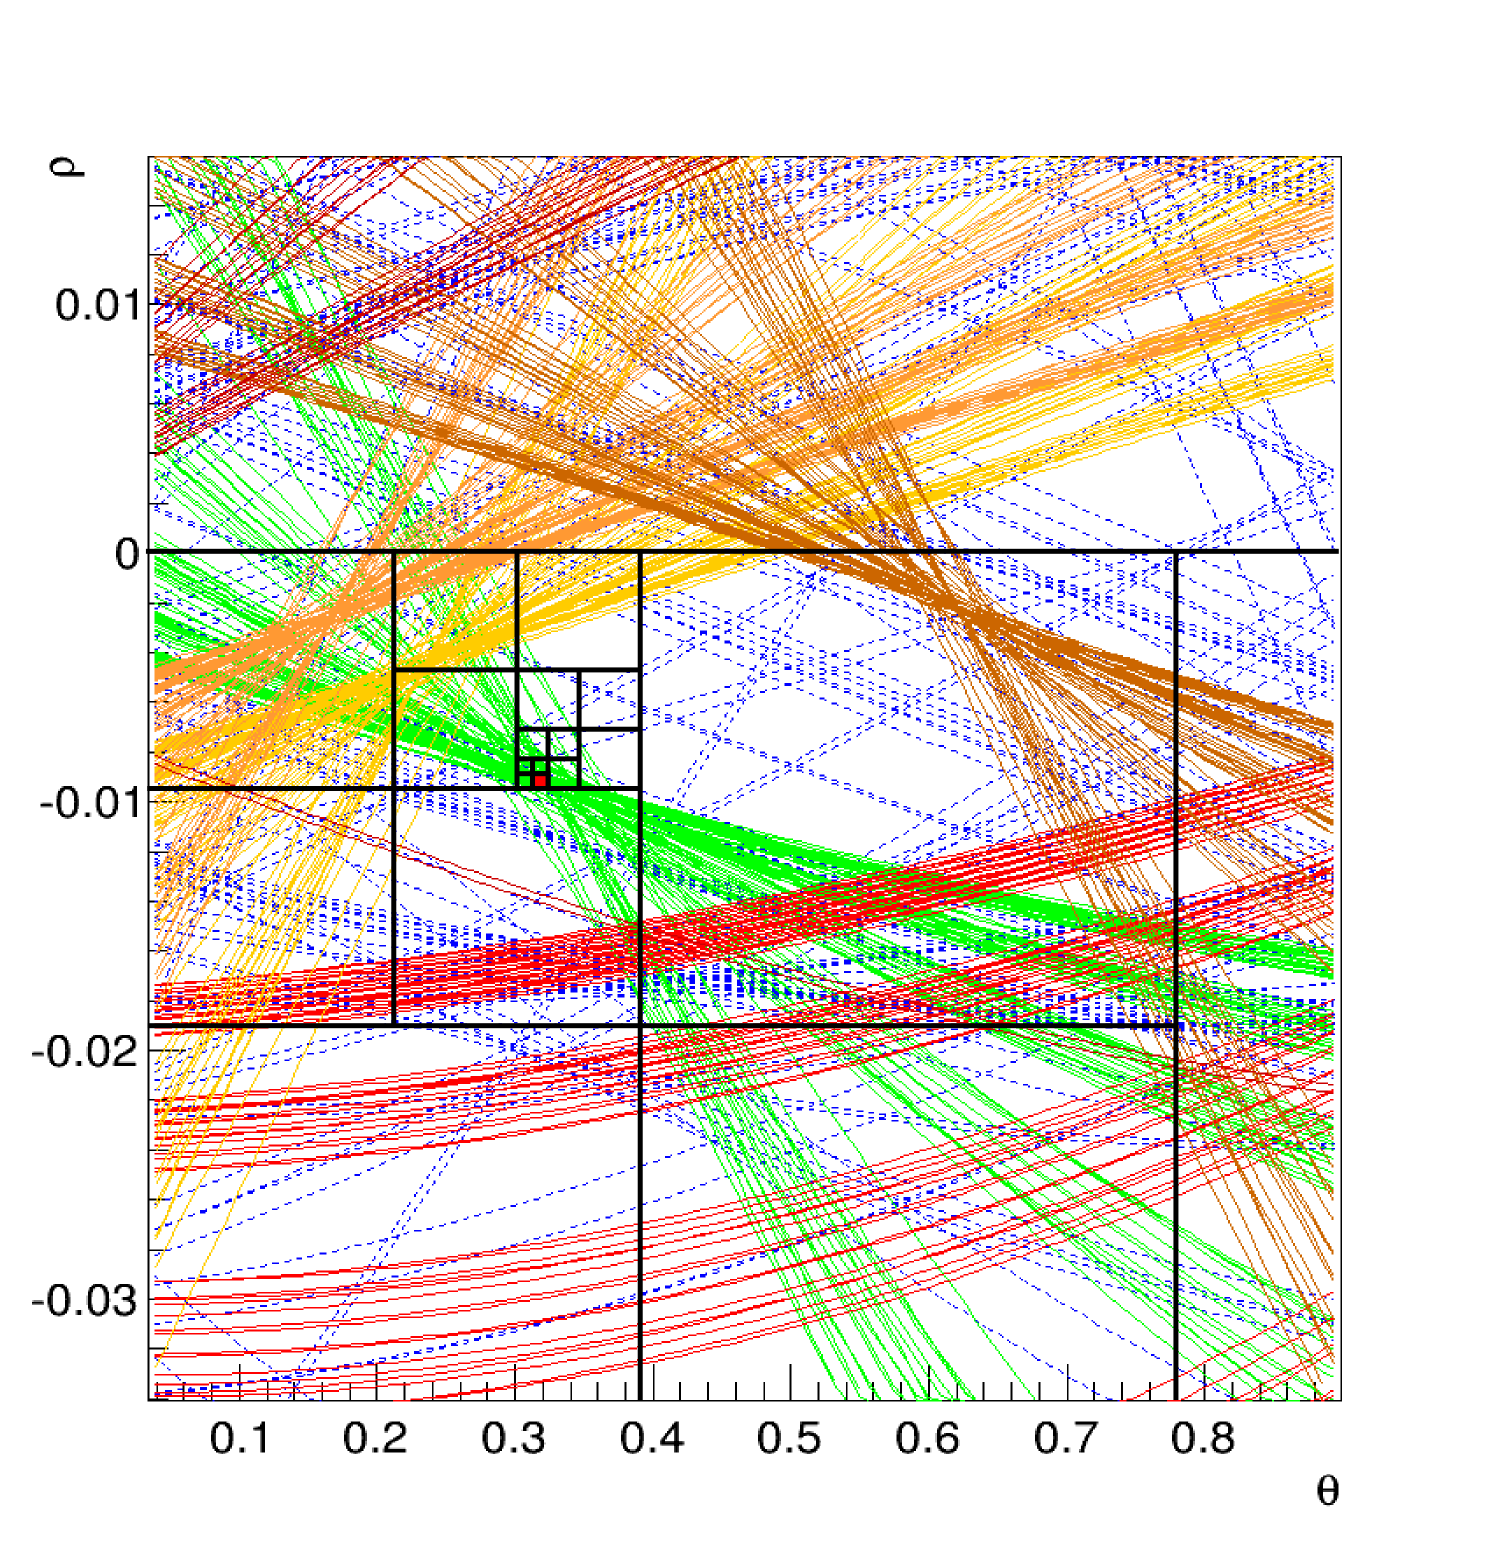
\includegraphics[width=0.5\linewidth]{figures/theory/quad_tree.png}
  \caption[Quad tree search.]{Depiction of a quad tree search to find the bin with the most interceptions of sinograms shown in the smallest box in the center. Only the first round of the search without multicandidate search is shown for better visibility. Each color shows sinograms that belong to the same charged particle. Taken from~\cite{viktor_dpg}.}
  \label{fig-quad-tree-search}
\end{figure}


\subsubsection{Stereo Hit Finding}

In this thesis a refined algorithm for assigning stereo hits was implemented. The aforementioned Legendre track finding algorithm does only work for axial hits, as a precise position in $x$ and $y$ is needed for calculating the position in the Legendre space. Therefore it can not be applied for hits coming from stereo wires as they have a certain range of possible $x$--$y$-coordinates. But as soon as trajectories is found using only axial hits, for each of those candidates matching stereo hits can be reconstructed to fit the trajectory in such a way that its drift circles touch the trajectory circle of the candidate. This is only possible for a fraction of the stereo hits given an axial trajectory, as the stereo wires have only a small tilting angle. As a stereo wire can be best approximated by a single line in 3d space the $z$ position is now also fixed. It is not possible to gain information on whether the drift circle is included in the trajectory circle or not -- for the same reason there were two sinograms. Therefore each stereo hit leads to two slightly different reconstructed $z$ positions. 

An ideal trajectory in the $s$-$z$ plane, with $s$ being the travel length in the circular two-dimensional projection, resembles a straight line analogous to the circle in the $r$--$\phi$ plane and can again be described by two parameters. This time these parameters are the slope\footnote{It is described by the angle $\lambda$ for consistency with the helix parameters used for track parametrization.} $\tan \lambda$ and the distance $z_0$ on the $z$-axis to the interaction point. The plane spanned by these two parameters is analogous to the Legendre space in the axial case. As before each point corresponds to a certain trajectory. By using both reconstructed $z$ values from each stereo hit, two functions in this plane can be drawn which include every possible trajectory that would have passed the stereo hit. For axial hits these functions were given by the two sinograms. For stereo hits they are straight lines in the $\tan \lambda$--$z_0$-plane:
$$ z_0 = z_\text{rec} - \tan \lambda \cdot s_\text{rec} $$
with the reconstructed $z$ positions $z_\text{rec}$ and the reconstructed travel distance $s_\text{rec}$ which can be calculated using trigonometrical relations as the trajectory in a two-dimensional plane with fixed $z$ is approximated as a circle. The whole process can be seen in figure~\ref{fig-stereo-explained}. Again, a quad tree search is applied to search for the point with the highest number of interceptions which corresponds to the trajectory parameters compatible with the largest number of hits. This time only the single highest trajectory is stored as one single trajectory in the $r$--$\phi$ plane can only have one single trajectory in the $r$--$z$ plane. The whole algorithm is repeated for all other found axial-only trajectories. 

For most of the particles the energy loss has no influence on the $s$--$z$ motion because a momentum change would lead to the same deviations in the $z$ and the $s$ motion leaving $\tan \lambda$ approximately identical. Additionally, a non-zero distance to the interaction point is already accounted for, so post-processing is not needed here. See chapter~\ref{chapter-workflow} on the \texttt{SegmentTrackCombiner} for a description of how to cope with the remaining inefficiencies.


\begin{figure}
 \centering
 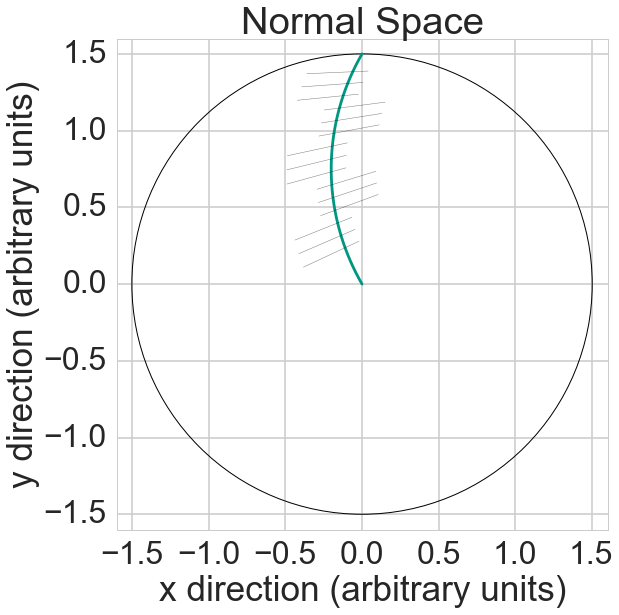
\includegraphics[scale=0.3]{figures/theory/stereo_1.png}
 \hspace*{1cm}
 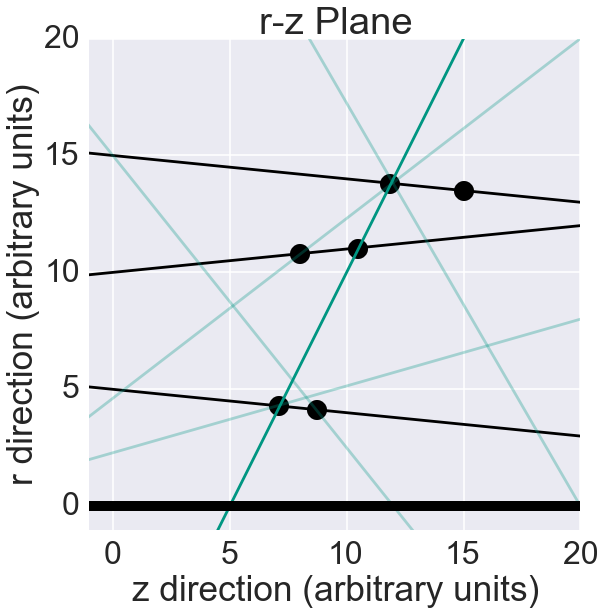
\includegraphics[scale=0.3]{figures/theory/stereo_2.png}
 
 \vspace*{1cm}
 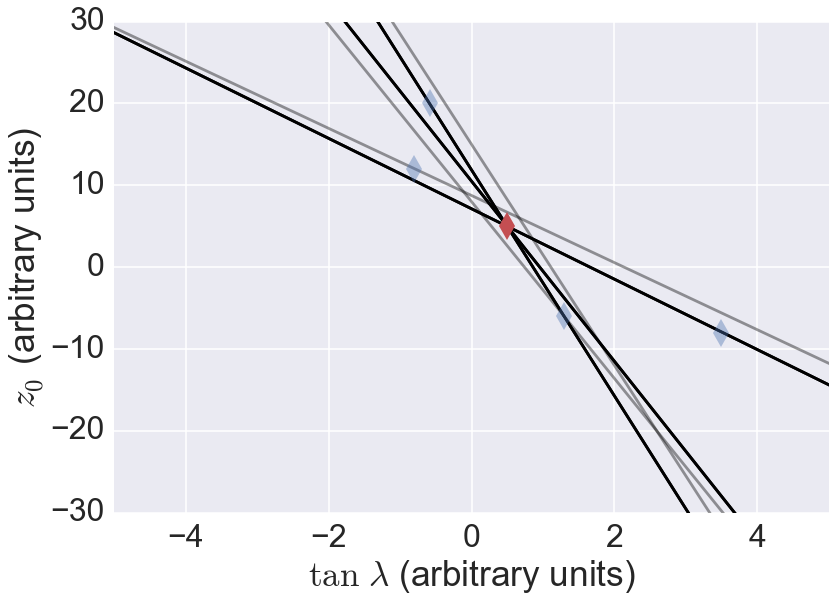
\includegraphics[scale=0.3]{figures/theory/stereo_3.png}
 \caption[Stereo Legendre algorithm.]{Stereo hit finding algorithm shown for a single track. The trajectory in the $r$--$\phi$ (left upper) plane leads to two possible $z$ positions for each stereo hit (right upper). On the left upper side the trajectory together with the stereo wires projected to the $r$--$\phi$ plane is shown. In principle each stereo hit could have been created by an infinite number of tracks. Some of them are shown in green in the right upper picture. The dark green track is the correct hypothesis. Each line corresponds to a single point in the $\tan \lambda$--$z_0$-plane, which is shown below together with the correct trajectory parameters as a red diamond. The green diamonds correspond to the wrong light green lines in the right diagram. The $\tan \lambda$-$z_0$-lines for each hit as described in the text are also shown in black (correct hits) or in dashed (wrong hits).}
 \label{fig-stereo-explained}
\end{figure}


\subsection{The Automaton Track Finder}
Before doing the quad tree search, the Legendre algorithm transforms each hit to the Legendre space in the same manner making it a global hit finder. The automaton track finder however is a local track finding algorithm using the neighborhood relations among the hits. It processes the hit information in two stages:
\begin{zlist}
  \item Clusterize the hits into groups and create segments out of these clusters. A segment is a smaller part of a track limited by the superlayer bounds of the CDC.
  \item Use these superlayer segments and combine them into track candidates.
\end{zlist}

Both steps include the same problem: find the correct candidate among all combinations of items in a set. In the first step, these items are the hit clusters, in the second step the segments. In both cases the problem is solved by applying a cellular automaton algorithm which is described briefly in the following. More information can, for example, be found in~\cite{cats},~\cite{kisel} and~\cite{oliver}. Each element in the set of items to be combined is modeled as a node in an acyclic directed graph. The edges in this graph represent the fact that a combination between adjacent elements is in principle possible. The implementation of this decision is of course dependent on the item type and the purpose of the cellular automaton. The graph is directed because the natural flight direction of the tracks introduces a preferred direction and acyclic because the number of particles passing the same wire twice without leaving the superlayer is negligible. The cellular automaton now seeks to find the longest path in this directed graph, i.e.\ the path passing the highest number of nodes. To have more finer control on the output of the algorithm one can also apply weights to the edges and nodes of the graph. The output path is now not necessarily the longest path but the path with the highest sum of weights of the included edges and nodes. The cellular automaton algorithm finds this path by recursively traversing through the nodes and searching for the path with the highest sum of weights starting with this node. By passing this information to all parent nodes the output path can be easily found. The process is depicted in figure~\ref{fig-automaton}. If one is not only interested in the single best path, this procedure is repeated with the previously used items removed from the graph.

\begin{figure}
  \centering
  \begin{tikzpicture}[thick]
    \def\h{1}
    \def\x{2}
    
    \node[fill=kit-green50] (1) {1};
    
    \node[right=\x of 1] (dummy1) {};
    \node[fill=kit-green50, above=\h of dummy1] (2) {2};
    \node[fill=kit-green50, below=\h of dummy1] (3) {3};
    
    \node[fill=kit-green50, right=\x of dummy1] (4) {4};
    
    \node[right=\x of 4] (dummy2) {};
    \node[fill=kit-green50, above=\h of dummy2] (5) {5};
    \node[fill=kit-green50, below=\h of dummy2] (6) {6};
    
    \node[right=\x of dummy2] (dummy3) {};
    \node[fill=kit-green50, above=\h of dummy3] (7) {7};
    
    \draw[vecArrow, kit-orange50] (1) -- (2) node  [midway, sloped, above] {2.3};
    \draw[vecArrow] (1) -- (3) node  [midway, sloped, above] {1.7};
    \draw[vecArrow, kit-orange50] (2) -- (4) node  [midway, sloped, above] {0.6};
    \draw[vecArrow] (4) -- (5) node  [midway, sloped, above] {0.2};
    \draw[vecArrow, kit-orange50] (4) -- (6) node  [midway, sloped, above] {3.3};
    \draw[vecArrow] (5) -- (7) node  [midway, sloped, above] {0.1};
\end{tikzpicture}
\caption[Cellular automaton.]{Picture showing a typical acyclic directed automaton with nodes (green boxes) and edges (arrows) with their weights (number on the arrows). The algorithm outputs the orange path although the path 1-2-4-5-7 includes more nodes because its sum of weights is larger.}
\label{fig-automaton}
\end{figure}

The first step of the automaton track finder is to clusterize the hits into sets. A cluster of hits is defined as the largest set of directly adjacent hits in a single superlayer. This condition can also be weakened to allow for one-cell-wide gaps in the clusters. A typical event display with the found clusters is shown in figure~\ref{fig-clusters}. The segments which are built next are fully contained in one single cluster -- but one cluster can contain more than one segment when two tracks cross each other in this superlayer. To decide from which partition of hits in a cluster the segment should be built, the cellular algorithm is applied independently for each cluster. The nodes in the graph are given by the so-called facets. One facet is one of the possibilities of assembling three wire hits with those hits pairwise in close proximity to each other in two cases. Three possibilities for facets are shown in figure~\ref{fig-facets}. As can be seen in the figure, each wire hit already has a left-right passage information attached to it and combinations of the same three wires with different left-right information form different facets. With this left-right information a direction of flight can be defined (except for the sign). Configurable filters are used to trim down the created three-hit combinations to only compatible facets by limiting, for example, the angular deviation between the tangents to pairs of hits. Before applying the cellular automaton one also has to define the edges of the graph. Two facets have a directed connection in the graph if and only if the second and third hit of the first facet resemble the first and second hit of the second facet together with its left-right information and the angle between the defined directions of flight does not exceed a certain threshold. After performing the cellular automaton algorithm a set of paths including those facets is obtained. By collecting the hits included in those paths segments can be built.

\begin{figure}
  \centering
  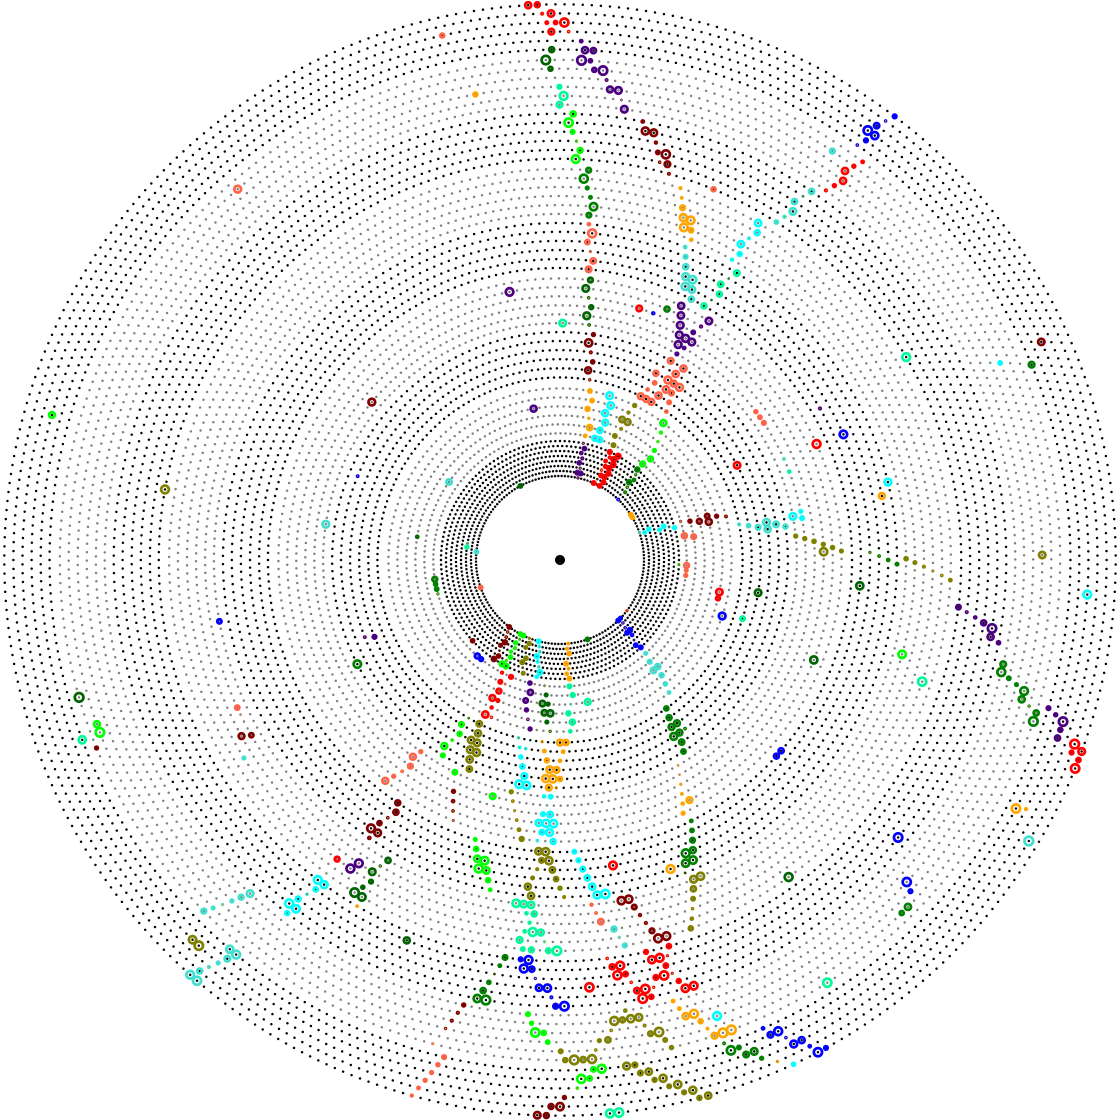
\includegraphics[width=0.8\linewidth]{figures/theory/clusters.png} 
  \caption[Clusters in the automaton track finder.]{A typical event with colored clusters. The different colors have no particular meaning and are only for better distinction.}
  \label{fig-clusters}
\end{figure}

\begin{figure}
  \centering
  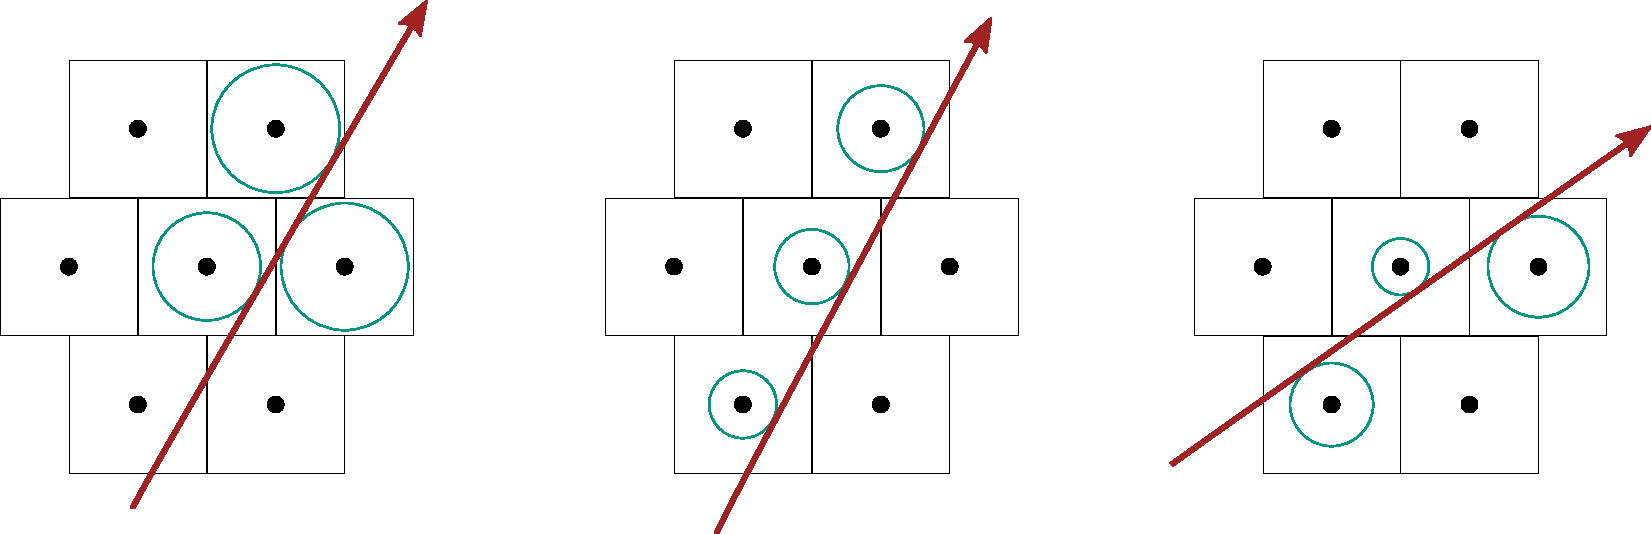
\includegraphics[width=\linewidth]{figures/theory/facets.pdf}
  \caption[Facets used in the automaton track finder.]{Three possibilities for facets with corresponding tangents (shown as red arrows) made from wire hits (in green). When changing the left-right hypothesis of one of the wire hits (which is not shown here) the facet is different than before. The sign of the direction vector can not be obtained with this local information. Taken from~\cite{oliver}.}
  \label{fig-facets}
\end{figure}

To construct the direction of flight and the tangents a distinct $x$-$y$ position for each hit is needed. For axial hits this position is given by the wire position, but stereo wires, in the absence of the $z$ position, do not have fixed coordinates in this plane. The problem can be solved by using the positions of the stereo wires for $z = 0$ in the cellular algorithm. This does not produce a large error as the reciprocal position of the stereo hits in one layer does not change much with different $z$ positions.

In this thesis, different possibilities of combining the results of the Legendre track finder with the ones coming from the automaton track finder are investigated and implemented. For most of the cases, the produced segments are used instead of full tracks for reasons described in later chapters. In order to run the local track finder as a standalone algorithm, the second step of creating track candidates out of the produced segments is also necessary. As this step is also performed using the cellular algorithm procedure the identities of nodes and edges have to be defined again. One natural choice would be to use the segments for the nodes and connect each pair of segments in the graph directly if their distance is small enough. Another approach is to use pairs or even three segments lying in consecutive superlayers. These groups of segments contain at least one stereo segment, giving the track piece $z$-information. This $z$-information can be used to create relations between those segment groups. Running the cellular automaton in a multipass manner leads to a collection of track candidates.


\section{Figures of Merit}

For testing and developing and also for later usage in a physics analysis, numbers from the implemented track finding algorithms need to be compiled to see how well they work. There are three main classes of figures of merit to describe a track finding algorithm. All three classes listed here are described in more detail below. The three classes are:
\begin{itemize}
  \item efficiency (e.g.\ the hit or finding efficiency, also for different particle types, momentum regions or areas in the detector)
  \item error rate (e.g.\ the clone or fake rate)
  \item computational performance (e.g.\ timing and memory consumption)
\end{itemize}

The last class should be quite clear and is measured by the basf2 measuring algorithms. As the tracking is part of the reconstruction chain and may be at some point adopted for the high level trigger, the timing performance is very important. 

The other two classes can best be described by the algorithm that computes them. It starts with a Monte Carlo (MC) simulation of generic $\PB\APB$ events with the full detector simulation afterwards. The created hits can then be grouped into distinct sets -- each describing a simulated track, called MC track candidate or MCTrackCand\footnote{They are also called track candidates to fit the naming convention of the track finder, although they are not candidates but rather correct tracks.}. Only those tracks that have at least 3 hits in the CDC are kept as a MCTrackCand -- otherwise they can not be fitted and even if there was a chance to find them via track finding, they could not be used for physics analyses because of the low resolution of their parameters. After that, the simulated hits are used for track finding with the method to be evaluated. This can be done easily as the simulated hits are transformed into a format that is similar to the format that will be used later for the data recorded by the experiment. After the track finder has produced a list of track candidates also, we can use the saved MC information to match tracks from the track finder to tracks from the MC algorithm by counting the number of hits they share. The different cases are depicted and described in table~\ref{tab-mc-track-finder}.

\begin{table}
  \centering
  \begin{tabular}{m{0.4\linewidth}m{0.5\linewidth}} \toprule
    \centering 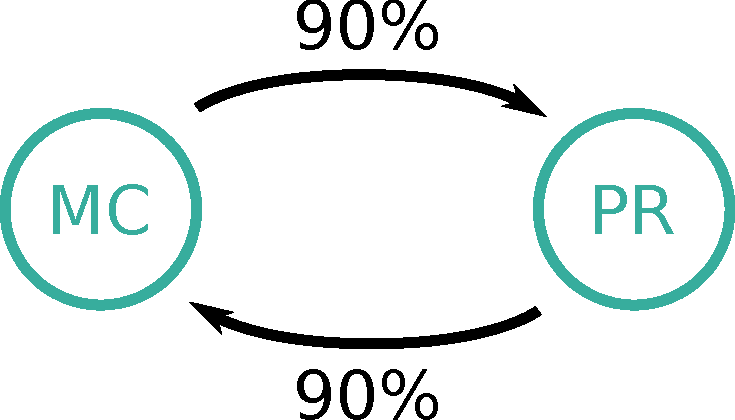
\includegraphics[width=0.8\linewidth]{figures/theory/fom_found.pdf} & There is a one-to-one connection between a MCTrackCand and a track from the track finder. The MCTrackCand is labeled found and the other track is labeled matched. \\ \midrule
    \centering 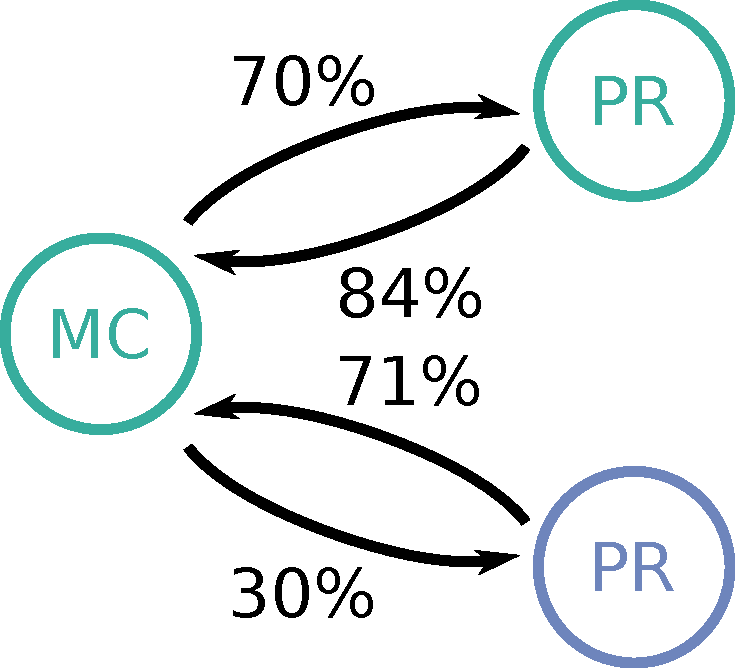
\includegraphics[width=0.8\linewidth]{figures/theory/fom_clone.pdf} & The MCTrackCand is found twice. The track from the track finder with the highest percentage (the green one in this example) is labeled matched, the other one is labeled cloned. The MCTrackCand is nevertheless labeled found. \\  \midrule
    \centering 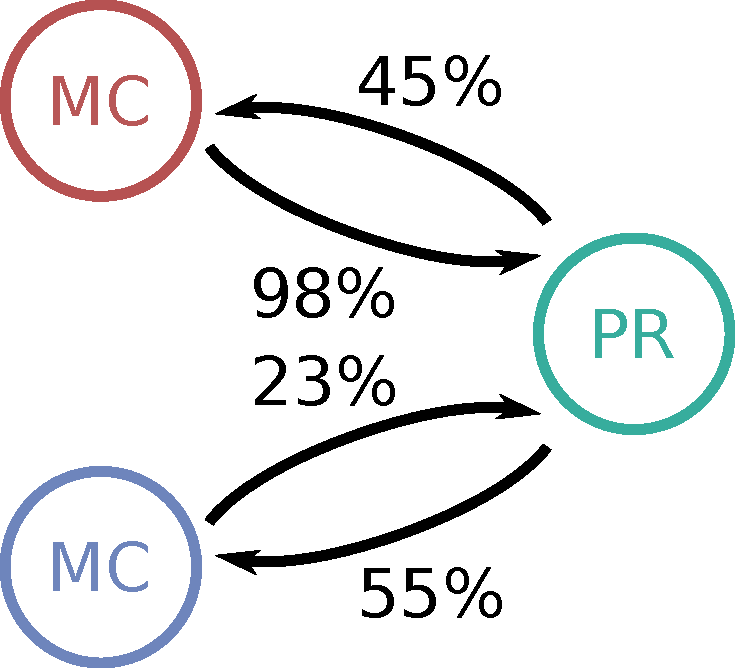
\includegraphics[width=0.8\linewidth]{figures/theory/fom_fake.pdf} & The track from the track finder is created with hits from many different MCTrackCands. As none of the corresponding hit ratios exceeds 66 \%, the PR track is called fake. The value 66 \% is a rather arbitrary value, but is chosen in a way to give a good estimate on the number of fakes. The hit ratios of the MCTrackCands itself do not play any role here. \\  \midrule
    \centering 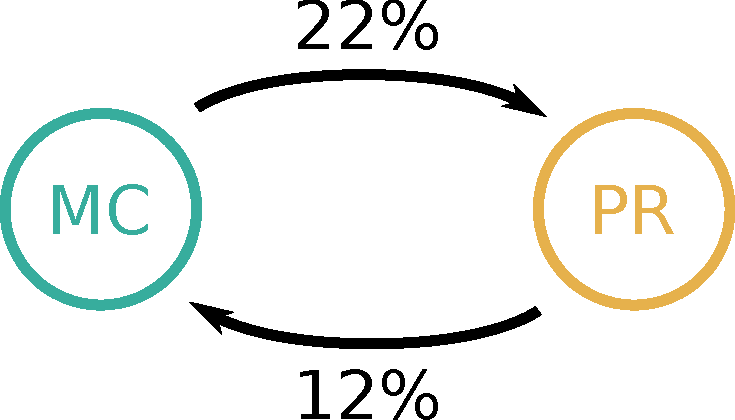
\includegraphics[width=0.8\linewidth]{figures/theory/fom_background.pdf} & The found track does not describe any of the MCTrackCands well (or well enough) -- but is made out of background hits. This track is also called a fake. \\ \bottomrule
  \end{tabular}
  \caption[Matching routine for compiling the FOM.]{This table shows the four different cases for the matching between MCTrackCands (MC, shown on the left side of the pictures) and tracks found by the pattern recognition algorithm (PR, on the right side). The different colors differentiate between different tracks. Aan arrow between tracks shows that these two tracks share hits. The two percentages on the arrows are the percentages of hits they share in respect to the total number of hits in the MCTrackCand (arrows from MC to PR) or in the track candidate from the track finder (from PR to MC).}
  \label{tab-mc-track-finder}
\end{table}

The finding efficiency describes the rate of MCTrackCands which are labeled matched to the total amount of MC track candidates. Building this ratio can also be done for bins in various variables, e.g.\ perpendicular momentum ($p_T$), angle in the curling plane ($\phi$), number of tracks per event (multiplicity) and many more. A perfect track finder would have a finding efficiency of 100 \%. In most of the cases, the finding efficiency drops for tracks in a certain region of these variables -- e.g.\ low momentum tracks.
The hit efficiency is the mean of the ratios between the number of hits in the MCTrackCands matched to a non-fake track candidate to the number of hits in total of this track. A perfect track finder would have also a hit efficiency of 100 \%. In most of the cases the hit efficiency drops because of energy losses and deviations from the perfect trajectory form due to multiple scattering.
The fake and clone rates are the number of track candidates labeled as fake or clone by the matching algorithm divided by the number of found tracks in total. A perfect track finder would achieve both number at 0 \%. A high fake rate is caused by a track finder with too loose cuts when putting together single pieces of tracks to one big track or by one which often picks up background hits. A track finder with a high clone rate on the other hand has too harsh cuts and often splits up tracks into more than one piece. To reduce statistical errors, these figures of merit are calculated for a high number of events.

\section{Track Fitting} \label{section-fitting}

Track finding algorithms have the task to partition the measured hits into sets with each set forming a track candidate. Afterwards the purpose of a track fitting algorithm is to fit a model for the trajectory to the measured information of the hits to gain the particles properties, e.g.\ the momentum and position. The model used for the fit can be very simple without taking into account material effects or energy loss. The track fitting algorithms implemented in genfit2~\cite{genfit} -- one of the external libraries used in basf2 -- however takes care of the interaction of the particles with material by using the same algorithms in calculating these material effects that are used for simulating the detector geometry. As the calculation itself depends strongly on the track parameters this implies recalculating the material effects of the particle with every fitting step. Therefore an algorithm like the Kalman filter with its iterative approach is well-suited for track fitting.

The Kalman fitter algorithm~\cite{kalman} is based on the idea of iteratively adding measurements (e.g.\ the positions of the hits associated with this track) to the current state of the trajectory. Therefore the parameters change with every newly added hit and should, in principle, converge to the correct trajectory parameters. By extrapolating a model of the trajectory with the current parameters to the plane of the next hit measurement, new predictions are calculated. The information of these predicted and the measured hits weighted by their responsible errors are used to compute a refined track state. By transversing back and forth several times through the whole hit set the final parameter estimation is found. One step in this procedure with only a small hit set is depicted in figure~\ref{fig-kalman}. As described before, the Kalman algorithm needs a current parameter state to calculate the extrapolation and the updated parameter set. As there is no possibility to gain a current parameter set before processing the first few hits the track finder must provide a starting seed for the track parameters.

\begin{figure}
 \centering
 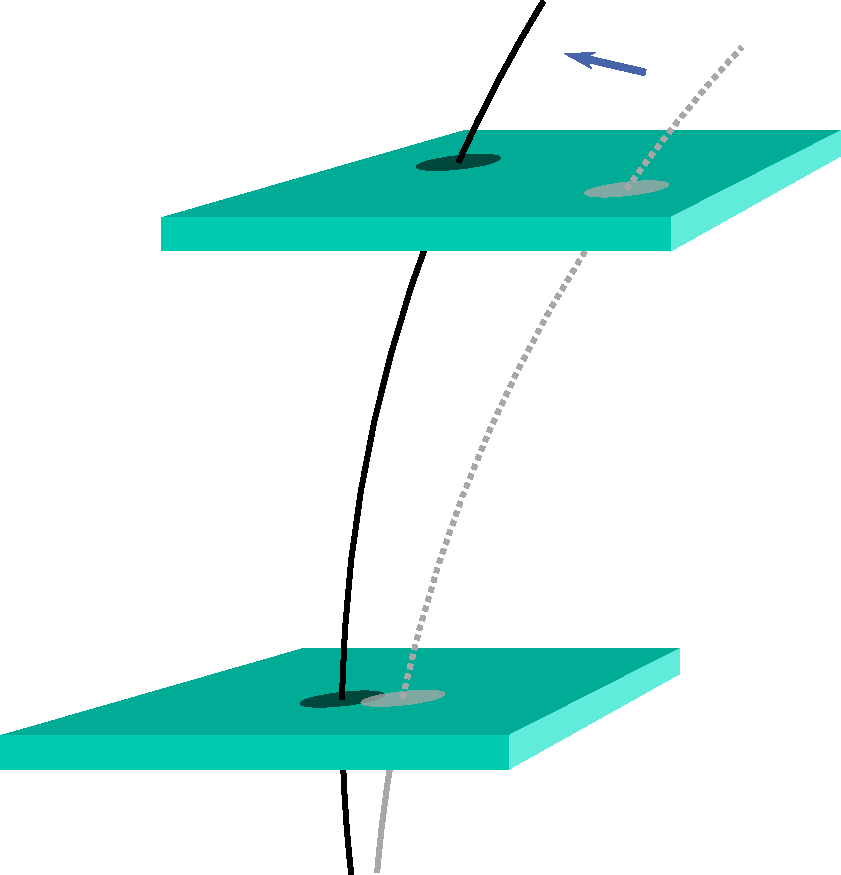
\includegraphics[width=0.6\linewidth]{figures/theory/kalman.pdf}
 \caption[One step of the Kalman fitter procedure.]{Sketch of one step in the Kalman fitter procedure. The real track parameters are depicted by the black trajectory. The green planes represent two sensors. The track passage positions -- the hit position measurements -- are shown as black circles. The current state of the fitting parameters is shown in gray. The state is extrapolated from the lower to the upper plane (gray dashed) and a new reconstructed position is calculated (gray circle on the upper plane). As there is a deviation between the current and the measured hit position, the current trajectory is changed according to the blue arrow.}
 \label{fig-kalman}
\end{figure}

When taking into account fake or background hits in a track, the Kalman fitter algorithm may not lead to good results anymore. As each hit is used for estimating the parameters of the trajectory a wrongly attached hit can give a wrong bias on these parameters. Therefore a weighting scheme is applied to all hits after each Kalman pass and this weight defines how strong one hit affects the final parameters. There are many different ways to do so, including elastic tracking and nonlinear filters~\cite{daf_fruh}. The one currently used for the tracking in the Belle~II software framework is the \emph{deterministic annealing filter} (DAF) introduced by Frühwirth and Strandlie. The procedure is as follows:
\begin{zlist}
  \item Set the weights of all hits to 1.
  \item Fit the track with a Kalman fitter taking into account the weights of each hit. \label{list-daf-loop-start}
  \item Recalculate the weight of each hit with the distance of the hit to the current trajectory hypothesis.
  \item Dismiss hits with a weight below a certain threshold.
  \item Continue with (\ref{list-daf-loop-start}) until a defined number of iterations is reached or the fit is converged.
\end{zlist}

To overcome the difficulties of badly chosen starting parameters of the fit that would lead to dismissing a large number of hits in the first iteration an annealing scheme is applied: each weight is transformed with a Maxwell-Boltzmann distribution depending on a ``temperature'' $T$ which is decreased with every iteration. In the first few iterations, with a high temperature, hits with a small weight are kept while in later iterations these hits are dismissed.

The fitting procedures are implemented in basf2 with the external library genfit2~\cite{genfit} -- a library for generic and experiment-independent track fitting. Only a small interface for accessing the genfit2 procedures from the basf2 code is implemented. See chapter~\ref{chapter-vxd} on the VXD momentum estimation for more information on this topic.

\section{Multivariate Classification}

During track finding -- especially in post-processing procedures -- many decisions must be made: whether a hit belongs to a track, whether two tracks should be merged, whether a track should be dismissed as fake, etc. In the context of inefficiencies and fakes due to background hits these decisions may depend on many input variables. Additionally there is the need to have a smooth transition between the two corner cases ``dismiss all'' and ``accept all'' to allow for subsequent optimization. This problem of deciding between two different possibilities for each input element (for example each track) is called a classification problem in statistics and there are many ways to deal with such problems (see for example references~\cite{cowan} or~\cite{blobel}). For most of the classification tasks in the track finding package for the CDC detector a classification algorithm known as \emph{boosted decision tree} (BDT) is used. In the following the main features are described. See reference~\cite{friedman} for more information on the algorithm and reference~\cite{keck} for details of the implementation.

The task of a classification algorithm is to decide whether an input element described by a feature vector $\vec x$ belongs to one class of elements or the other -- often these classes are called the signal and the background class. The classifier maps the multidimensional feature vector $\vec x$ to a one-dimensional output variable -- often between 0 and 1 -- which is designed in a way to separate signal and background by mapping signal like data to values near 1 and background like data to values near 0. The output can therefore be transformed to a probability for the input data to look like a signal sample and a configurable cut on the output can be used to distinguish between the two classes with a configurable purity or efficiency.

A decision tree is one possible implementation of such a classifier. It is created by dividing the parameter space of the feature vectors $\vec x$ into small hypercubes. As this is done by applying a division in one variable at the time a tree structure like in figure~\ref{fig-decision-tree} is formed. Each input data sample can then be mapped to the signal fraction of the hypercube it belongs to which is the output of of the tree for this element. This signal fraction is determined with a training sample of Monte Carlo generated events with known classification information. The cut values and variables are chosen in such a way as to maximize a separation measure, e.g.\ the gini impurity that models the gain introduced by this separation. The measure is also calculated using the training sample.

Because the chosen cuts depend strongly on the training sample, a single decision tree can easily be overtrained. A classifier is called overtrained when its separation power on the testing data set is much better than on an independent testing sample because instead of generalizing the training data it fits its output function to the training data perfectly. An overtrained classifier can not classify anything else than those cases that were present in the training set. To avoid overtraining an algorithm known as boosting is applied to the decision tree. This algorithm creates a whole set of decision trees iteratively. Each decision tree is trained to separate the items classified wrongly by the one before. It does so by applying weights to the items. The final output of the classifier is a weighted sum of all single trees. By limiting the depth of a single decision tree it avoids overtraining but because of the huge number of trees it still has a great separation power.

\begin{figure}
  \centering
  \begin{tikzpicture}[thick]
    \node[module] (alldata) {Decision Tree};
    \def\h{1}
    \def\x{0.8}
    \node[module, text width=6em, fill=kit-orange50, below=0.25 of alldata] (cut1) {$x_3 > a$?};
    \node[below=\h of cut1] (dummy1) {};
    \node[below=\h of dummy1] (dummy2) {};
    \node[below=\h of dummy2] (dummy3) {};
    \node[module, text width=6em, fill=kit-orange50, left=3*\x of dummy1] (cut2a) {$x_1 > b$?};
    \node[module, text width=6em,fill=kit-orange50, left=\x of dummy2] (cut3a) {$x_7 > d$?};
    \node[module, text width=6em,fill=kit-orange50, left=5*\x of dummy2] (cut3b) {$x_5 > e$?};
    \node[module, text width=6em,fill=kit-orange50, right=3*\x of dummy1] (cut2b) {$x_2 > f$?};
    \node[module, text width=6em,fill=kit-orange50, right=\x of dummy2] (cut3c) {$x_4 > g$?};
    \node[module, text width=6em,fill=kit-orange50, right=5*\x of dummy2] (cut3d) {$x_6 > h$?};
    
    \node[module, text width=6em, left=\x of dummy3] (result3a) {10 signal events};
    \node[module, text width=6em, left=5*\x of dummy3] (result3b) {328 signal events};
    \node[module, text width=6em, right=\x of dummy3] (result3c) {4136 signal events};
    \node[module, text width=6em, right=5*\x of dummy3] (result3d) {4 signal events};
    
    
   \draw[vecArrow] (cut1) -- (cut2a.north);
   \draw[vecArrow] (cut1) -- (cut2b.north);
   \draw[vecArrow] (cut2a) -- (cut3a.north);
   \draw[vecArrow] (cut2a) -- (cut3b.north);
   \draw[vecArrow] (cut2b) -- (cut3c.north);
   \draw[vecArrow] (cut2b) -- (cut3d.north);
\end{tikzpicture}
\caption[Decision Tree.]{A decision tree dividing a 7-dimensional parameter space into 4 hypercubes with seven cuts in three layers. The last layer is used to generate the output of the decision tree by counting the number of signal events in this hypercube in the training sample.}
\label{fig-decision-tree}
\end{figure}


